\pagebreak
\subsection{Testing White box}
Effueremo testing white box tramite Branch coverage della seguente funzione:

\lstinputlisting[caption=Funzione da testare]{TestCases/funzioneWhiteBox.java}

\begin{center}
    \begin{figure}[h]
        \centering
        \caption{Grafo di copertura della funzione}
        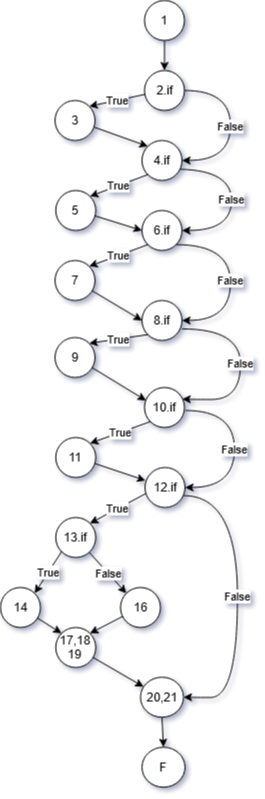
\includegraphics[height=0.9\textheight]{Figures/Grafo di copertura.png}
    \end{figure}
\end{center}


\lstinputlisting[caption=Casi di test]{TestCases/filtriUnitTesting.java}

\subsubsection{Ramo 2-3-5-7-9-11-13-21}
Il primo caso di test rappresenta una ricerca in cui l'utente non ha inserito nessun filtro e non ha attivato la ricerca per prossimità

\subsubsection{Ramo 2-...-15-18-19-21}
Il secondo caso di test rappresenta una ricerca in cui l'utente inserisce tutti i filtri ed ha attivato la ricerca per prossità

\subsubsection{Ramo 2-...-14-17-18-19-21}
Il terzo caso di test rappresenta una ricerca in cui l'utente inserisce tutti i filtri, ha attivato la ricerca per prossità e non ha inserito la distanza massima delle strutture rispetto alla posizione dell'utente.\\
\\
In questo modo abbiamo effettuato sia un branch coverage completo che un path coverage dei cammini linearmente indipendenti.\\ Tutti gli altri cammini risultano essere combinazioni lineari
dei cammini indipendenti già testati ed un loro test esaustivo richiederebbe 32*3 casi di test